\chapter{\texorpdfstring{Liveness}{Liveness}}
\label{ch:10}
\lecturemeta{Lezione 10 \quad\textbullet\quad 2026-07-03 \quad\textbullet\quad Roberto Bruni}{Petri nets · Esparza, \emph{Free Choice Petri Nets} (optional)}

In \hyperref[ch:09]{09 — Occurrence Graph} abbiamo imparato a costruire lo spazio degli stati raggiungibili e a chiederci se è finito (boundedness). Ora affrontiamo una domanda diversa, sul \emph{comportamento a lungo termine}: una data attività del processo \textbf{potrà sempre, prima o poi, essere eseguita}? Oppure può capitare di finire in uno stato da cui quell'attività non sarà \textbf{mai più} possibile? Questa è la nozione di \textbf{liveness} (vivacità), la proprietà chiave per garantire che un processo non "muoia" pezzo per pezzo. Studieremo la liveness delle transizioni, quella dei place, la nozione più debole di \textbf{deadlock-freedom}, e come queste proprietà si implicano a vicenda.

Una premessa logica utile per tutta la lezione: per \textbf{smentire} un'implicazione $P \Rightarrow Q$ basta esibire un caso in cui $P$ è vero e $Q$ falso, cioè

\[
P \wedge \neg Q
\]

E ricordiamo la transitività della raggiungibilità:

\[
M \in [M_0\rangle \ \wedge\ M' \in [M\rangle \ \implies\ M' \in [M_0\rangle
\]

Con "marcatura raggiungibile" intenderemo sempre "raggiungibile da $M_0$".

\section{\texorpdfstring{Liveness di una transizione}{Liveness di una transizione}}

Il primo istinto sarebbe dire che una transizione è "buona" se prima o poi si riesce a farla scattare. Ma questa è una condizione troppo debole: garantisce solo che $t$ scatti \emph{almeno una volta}, non che resti sempre possibile. La liveness chiede molto di più.

\begin{boxdefinition}{Live, dead, non-live, non-dead (transizioni)}
Una transizione $t$ può essere: - \textbf{live} (viva): può \emph{sempre} essere abilitata in futuro — qualunque cosa accada, non escludiamo mai che $t$ possa scattare di nuovo; - \textbf{dead} (morta): non potrà \emph{mai} più essere abilitata in futuro; - \textbf{non-live}: può \emph{diventare} dead (o lo è già); - \textbf{non-dead}: può essere abilitata \emph{almeno una volta}.
\end{boxdefinition}

L'aggettivo cruciale è \textbf{live}, e la sua definizione ha una struttura a due quantificatori che va letta con attenzione.

\begin{boxdefinition}{Transizione live (formale)}
Una transizione $t$ è \textbf{live} se da \emph{ogni} marcatura raggiungibile si può \emph{sempre} tornare a poterla abilitare: \(\forall M \in [M_0\rangle.\;\; \exists M' \in [M\rangle.\;\; M' \xrightarrow{t}\) Una rete è \textbf{live} se \textbf{tutte} le sue transizioni sono live.
\end{boxdefinition}

\begin{figure}[!htb]
\centering
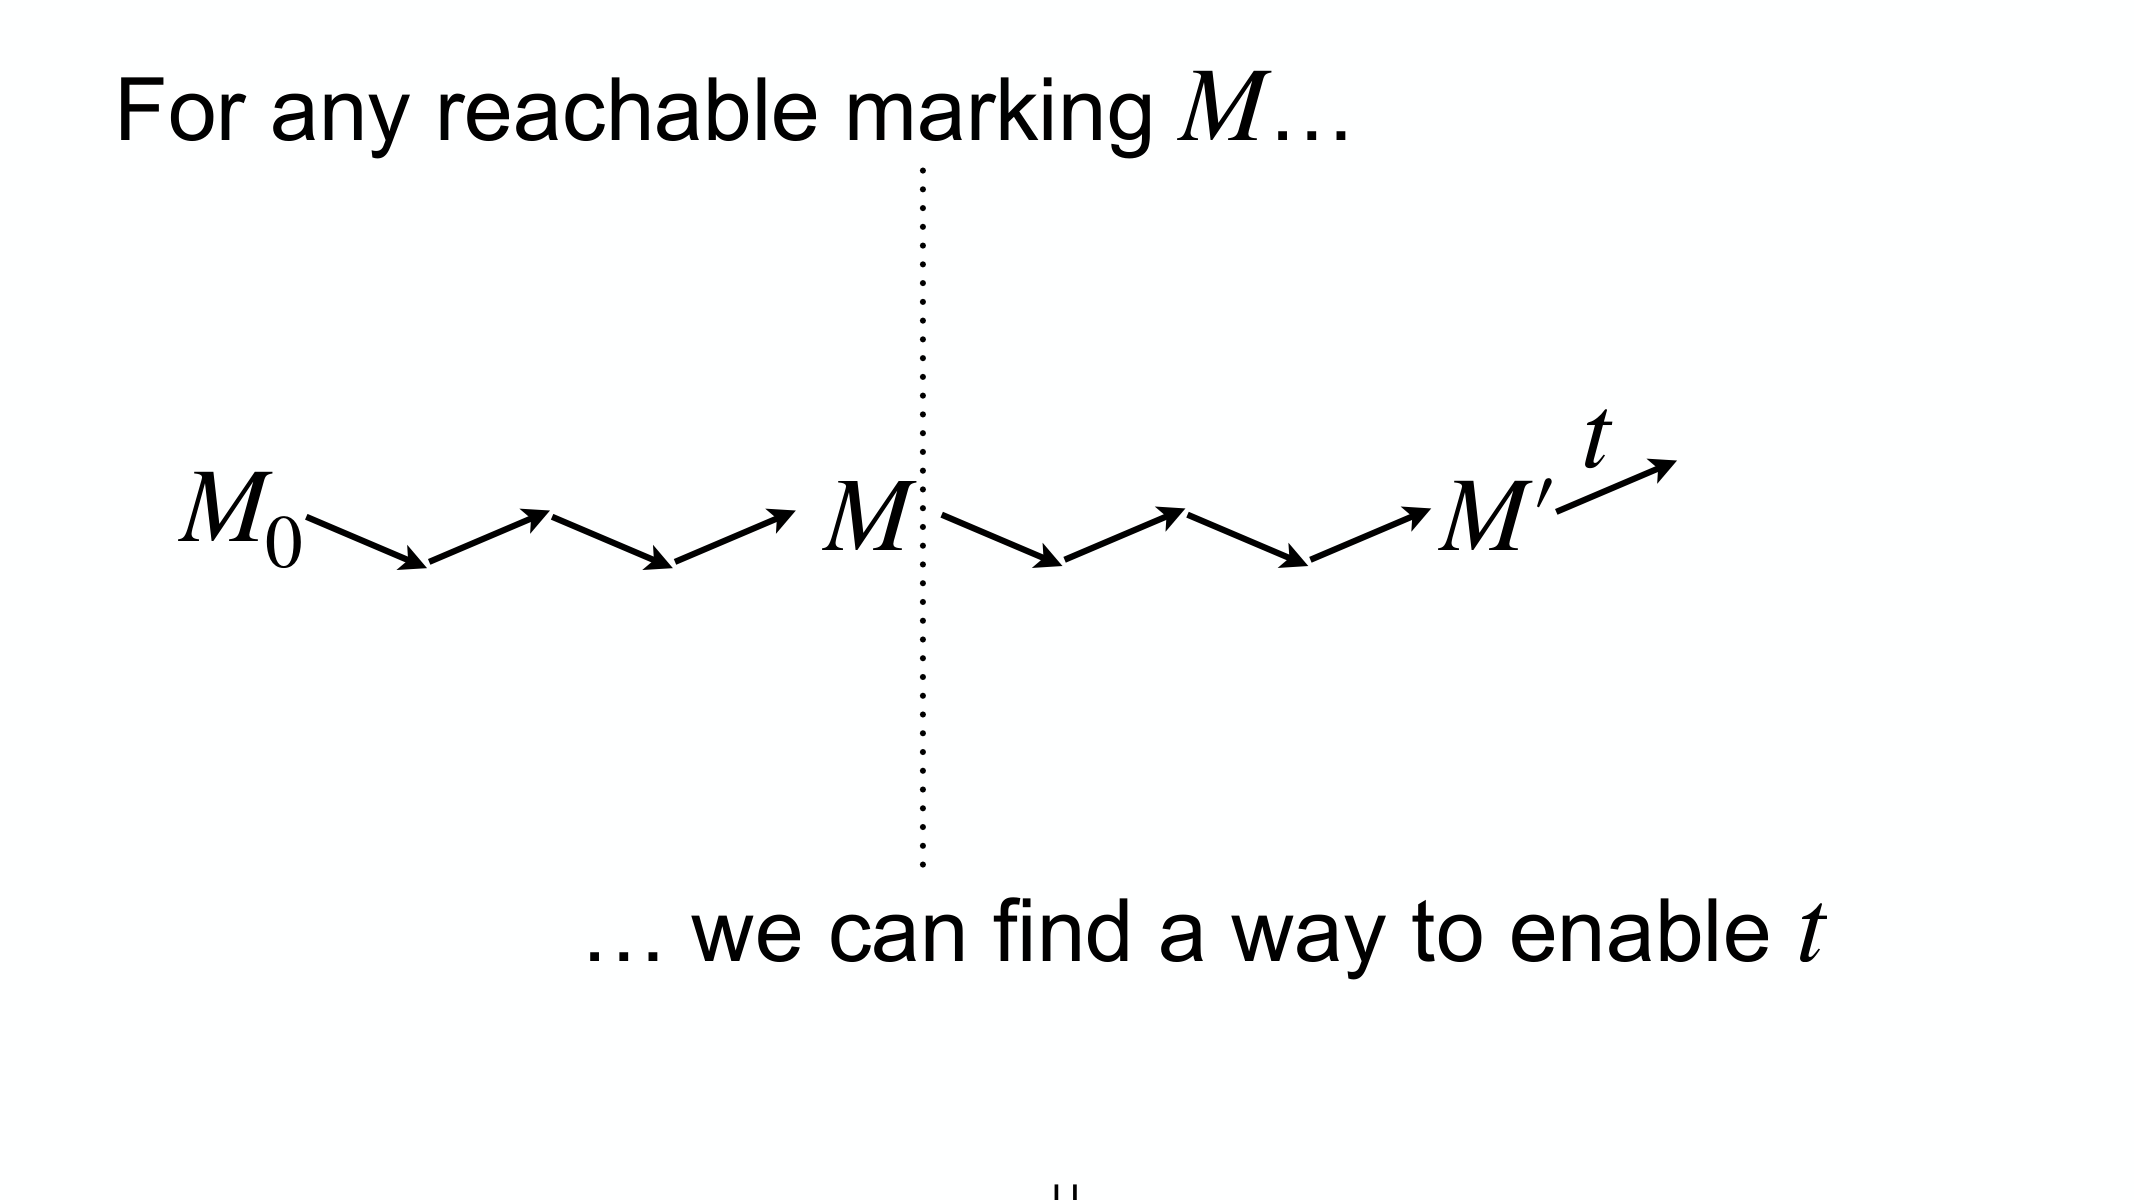
\includegraphics[width=0.74\linewidth,height=0.34\textheight,keepaspectratio]{images/10-liveness_p10_liveness-illustrated.png}
\caption{Liveness. \textbf{Per ogni} marcatura raggiungibile $M$ (parte sinistra), \textbf{esiste} un modo di proseguire fino a una marcatura $M'$ che abilita $t$ (parte destra). Il "per ogni... esiste" è il cuore: non importa dove sei finito, una via per riabilitare $t$ c'è sempre.}
\end{figure}

\begin{boxwarning}{Liveness $\neq$ "si può abilitare almeno una volta"}
Non confondere la liveness di $t$ con la proprietà, molto più debole, $\exists M \in [M_0\rangle.\; M \xrightarrow{t}$. Quest'ultima dice solo che $t$ \textbf{non è dead} al marking iniziale (si riesce a scattarla una volta partendo da $M_0$). La liveness invece pretende che, \textbf{da qualunque punto}, si possa \emph{ancora} riabilitarla. Una transizione può scattare all'inizio e poi morire per sempre: sarebbe non-dead ma \textbf{non} live.
\end{boxwarning}

Il modo migliore per afferrare la differenza è un esempio concreto, con marcature vere.

\begin{boxexample}{Una transizione che scatta e poi muore}
Prendiamo una rete lineare: $t_1$ prende il token da $p_1$ e lo mette in $p_2$, poi $t_2$ lo porta in $p_3$.

\begin{center}
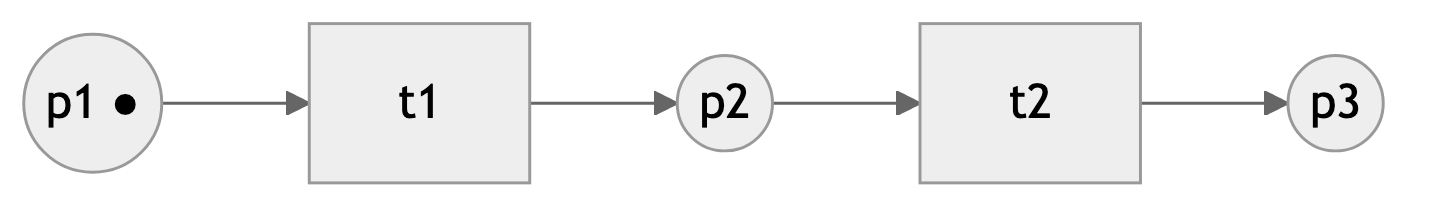
\includegraphics[width=0.74\linewidth,height=0.32\textheight,keepaspectratio]{images/mermaid/10_1.png}
\end{center}

Partendo da $M_0 = p_1$, le marcature raggiungibili sono solo $[M_0\rangle = \{\,p_1,\ p_2,\ p_3\,\}$ (il token avanza e basta). Verifichiamo $t_1$: - da $p_1$: $t_1$ è abilitata $\checkmark$; - da $p_2$: per riabilitare $t_1$ servirebbe un token in $p_1$, ma da $p_2$ si va solo verso $p_3$, mai indietro $\times$; - da $p_3$: fine corsa, niente scatta $\times$.

Quindi $t_1$ scatta \textbf{una volta} e poi non tornerà \textbf{mai più} abilitabile: è \textbf{non-dead} (ha scattato) ma \textbf{non live} (dalla marcatura $p_2$ è ormai dead). La condizione $\forall M \exists M'$ fallisce proprio su $M = p_2$: non esiste alcun $M'$ raggiungibile da $p_2$ che riabiliti $t_1$.

Per rendere $t_1$ \textbf{live} basterebbe chiudere un ciclo — es. una transizione da $p_3$ di nuovo verso $p_1$: allora da \emph{qualunque} marcatura si potrebbe sempre tornare in $p_1$ e riabilitare $t_1$.
\end{boxexample}

Le definizioni negate si ottengono \textbf{scambiando i quantificatori} ($\forall \leftrightarrow \exists$) e negando la condizione finale.

\begin{boxnote}{Recap formale (transizioni)}
\begin{itemize}
\item \textbf{Live}: da \emph{ogni} $M$ raggiungibile, \emph{esiste} un modo di riabilitare $t$.
\item \textbf{NonLive} (negazione): \emph{esiste} una marcatura $M$ da cui, comunque si prosegua, $t$ \emph{non} torna mai abilitabile.
\item \textbf{Dead}: $t$ non è abilitata in \emph{nessuna} marcatura raggiungibile (non scatta mai).
\item \textbf{NonDead}: $t$ è abilitata in \emph{almeno una} marcatura (scatta almeno una volta).
\end{itemize}

Il legame chiave è tra NonLive e Dead: la $M$ che testimonia la NonLive è una marcatura \textbf{da cui in poi $t$ è dead} (come $p_2$ nell'esempio). In una frase: \textbf{un sistema non è live $\Longleftrightarrow$ ha una transizione che a un certo punto può diventare dead.}
\end{boxnote}

Il modo pratico di verificare la liveness è sull'\textbf{occurrence graph}:

\begin{boxtip}{Liveness sull'occurrence graph}
\begin{itemize}
\item $t$ è \textbf{live} $\Longleftrightarrow$ da \emph{ogni} nodo del grafo si può raggiungere un nodo con un arco uscente etichettato $t$.
\item $t$ è \textbf{dead} (a $M_0$) $\Longleftrightarrow$ \textbf{non esiste alcun} arco etichettato $t$ in tutto l'occurrence graph.
\end{itemize}
\end{boxtip}

\section{\texorpdfstring{Liveness di un place}{Liveness di un place}}

La stessa idea si trasporta ai place, sostituendo "abilitata" con "marcato". Diciamo che un place $p$ è \textbf{marcato} in $M$ se $M(p) > 0$ (c'è almeno un token), \textbf{unmarked} se $M(p) = 0$.

\begin{boxdefinition}{Place live (formale)}
Un place $p$ è \textbf{live} se da ogni marcatura raggiungibile si può sempre tornare ad averlo marcato: \(\forall M \in [M_0\rangle.\;\; \exists M' \in [M\rangle.\;\; M'(p) > 0\) Intuitivamente: ogni volta che $p$ si svuota, resta la possibilità di rimarcarlo in futuro (o resta sempre marcato). Una rete è \textbf{place-live} se tutti i suoi place sono live.
\end{boxdefinition}

Come per le transizioni, $p$ è \textbf{dead} a $M$ se resterà unmarked per sempre:

\[
\text{Dead}(p) \equiv \forall M' \in [M\rangle.\; M'(p) = 0
\]

E sull'occurrence graph:

\[
p \text{ è live} \iff \text{da ogni nodo si raggiunge un nodo con un token in } p
\]

\[
p \text{ è dead} \iff \text{nessun nodo del grafo ha token in } p
\]

Escludiamo dal discorso i \textbf{nodi isolati} (place o transition con pre-set e post-set vuoti): consideriamo solo reti senza nodi isolati.

Vale la pena notare due fatti su come si propaga la "morte":

\begin{boxnote}{Come si propaga la deadness}
\begin{itemize}
\item I nodi dead \textbf{rimangono dead} in ogni marcatura successiva: l'insieme dei nodi morti può solo \textbf{crescere} durante un'esecuzione (non si "resuscita").
\item \textbf{Ogni transizione nel pre- o post-set di un place dead è a sua volta dead} (VERO): se $p$ resta sempre vuoto, le transizioni che lo consumano non possono scattare, e quelle che lo producono non possono scattare (altrimenti $p$ si marcherebbe).
\item \textbf{Non} vale il viceversa: un place nel pre- o post-set di una transizione dead \textbf{non è necessariamente dead} (FALSO): $p$ potrebbe essere marcato/smarcato da \emph{altre} transizioni.
\end{itemize}
\end{boxnote}

\section{\texorpdfstring{Liveness implica place-liveness}{Liveness implica place-liveness}}

Le due nozioni non sono indipendenti: la liveness delle transizioni è la più forte.

\begin{boxtheorem}{Live $\Longrightarrow$ place-live}
Se un sistema è live, allora è anche place-live.

\emph{Dimostrazione.} Prendiamo un place $p$ e una marcatura raggiungibile $M$; vogliamo trovare $M' \in [M\rangle$ con $M'(p) > 0$. Poiché la rete non ha nodi isolati, esiste una transizione $t \in \bullet p \cup p\bullet$ (che consuma o produce token in $p$). Per liveness, da $M$ si raggiunge $M''$ con $M'' \xrightarrow{t} M'''$. Ma allora $p$ è marcato \textbf{prima o dopo} lo scatto di $t$ (se $t \in p\bullet$ serviva un token in $p$ per scattare, se $t \in \bullet p$ lo produce): in ogni caso $M''(p) > 0$ oppure $M'''(p) > 0$, e abbiamo trovato la marcatura cercata. $\blacksquare$
\end{boxtheorem}

Il viceversa \textbf{non} vale: esistono reti place-live ma non live (un place resta sempre rimarcabile, ma una transizione può morire).

\section{\texorpdfstring{Deadlock-freedom}{Deadlock-freedom}}

C'è una proprietà più debole ma altrettanto importante: la garanzia che il sistema \textbf{non si blocchi del tutto}. Un blocco totale (deadlock) è una marcatura da cui \emph{nessuna} transizione può scattare — il processo è congelato.

\begin{boxdefinition}{Deadlock-freedom}
Una rete è \textbf{deadlock-free} se \emph{ogni} marcatura raggiungibile abilita \emph{qualche} transizione: \(\forall M \in [M_0\rangle.\;\; \exists t \in T.\;\; M \xrightarrow{t}\) Cioè: in qualunque momento dell'esecuzione, c'è \textbf{sempre almeno una} mossa disponibile. Sull'occurrence graph: \textbf{ogni nodo ha almeno un arco uscente}.
\end{boxdefinition}

\begin{figure}[!htb]
\centering
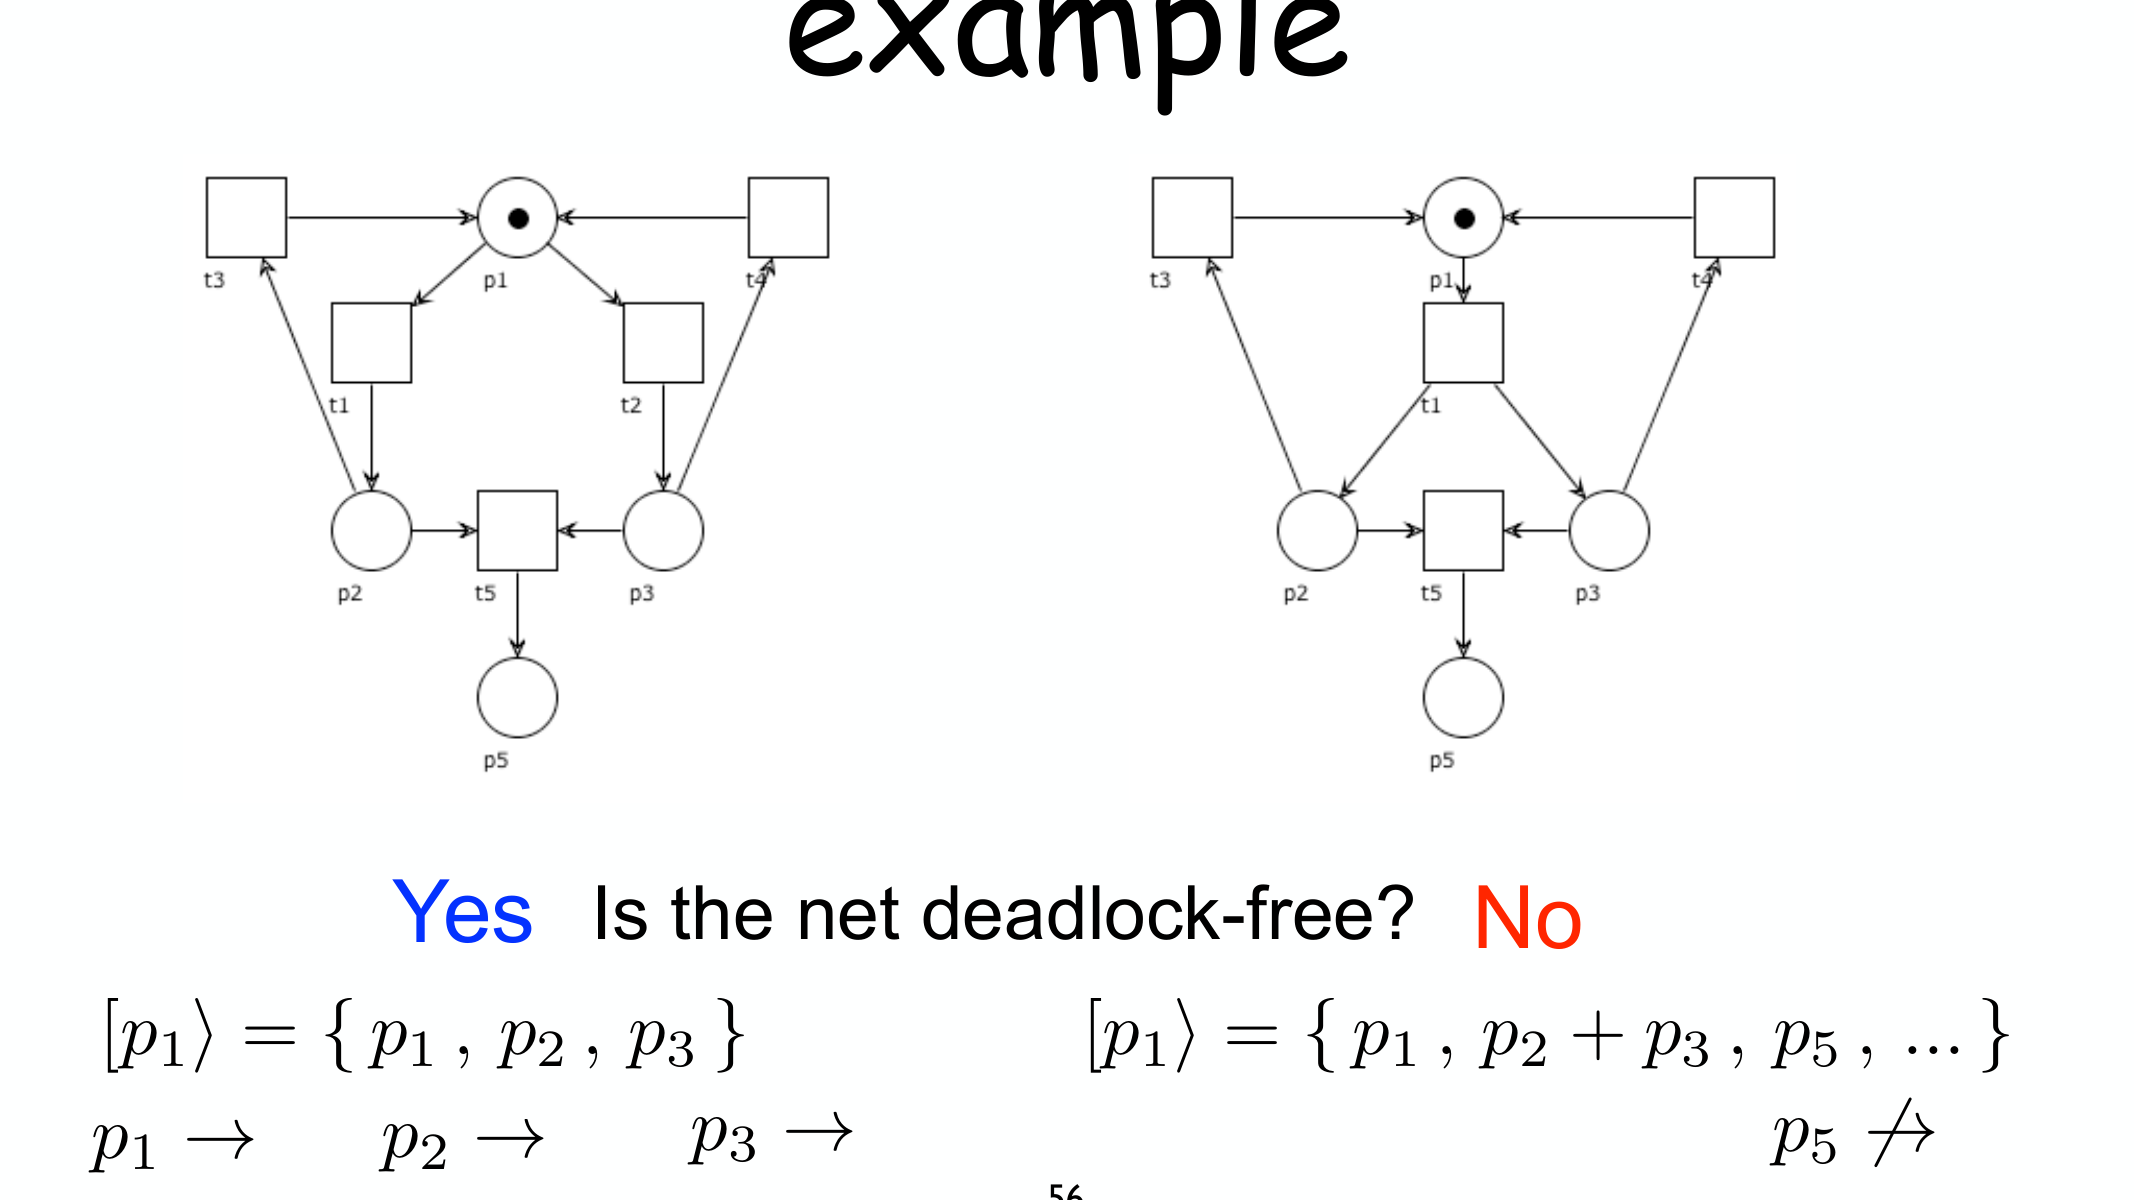
\includegraphics[width=0.74\linewidth,height=0.34\textheight,keepaspectratio]{images/10-liveness_p55_deadlock-free.png}
\caption{Deadlock-freedom. La rete di sinistra è deadlock-free: ogni marcatura raggiungibile abilita qualcosa. Quella di destra \textbf{no}: si può raggiungere una marcatura (es. con un token in \texttt{p5}) da cui \texttt{p5} non abilita alcuna transizione — il sistema è bloccato.}
\end{figure}

\begin{boxwarning}{Attenzione: deadlock $\neq$ non-live}
Deadlock-freedom è \textbf{più debole} della liveness. La liveness chiede che \emph{ogni singola transizione} resti sempre riabilitabile; la deadlock-freedom chiede solo che \emph{qualche} transizione sia sempre abilitata. Un sistema può girare all'infinito (deadlock-free) pur avendo una transizione che non scatterà mai più (non-live).
\end{boxwarning}

\section{\texorpdfstring{Il quadro delle implicazioni}{Il quadro delle implicazioni}}

Mettendo insieme i risultati si ottiene una gerarchia di proprietà, dalla più forte alla più debole. Il \textbf{lemma} centrale è che la liveness implica la deadlock-freedom.

\begin{boxtheorem}{Live $\Longrightarrow$ deadlock-free}
Se $(P,T,F,M_0)$ è live, allora è deadlock-free.

\emph{Dimostrazione (per assurdo).} Supponiamo esista $M \in [M_0\rangle$ con $M \not\to$ (deadlock). Prendiamo una transizione $t$ (l'insieme $T$ non è vuoto). Per liveness, esiste $M' \in [M\rangle$ con $M' \xrightarrow{t}$. Ma se $M$ è un deadlock, l'unica marcatura raggiungibile da $M$ è $M$ stessa ($[M\rangle = \{M\}$), quindi $M' = M$ e avremmo $M \xrightarrow{t}$: assurdo, perché $M$ era un deadlock. $\blacksquare$
\end{boxtheorem}

Un altro tassello: \textbf{place-live $\Longrightarrow$ deadlock-free} (se ogni place è sempre rimarcabile, da ogni marcatura si può muovere qualcosa). Riassumendo tutte le relazioni:

\begin{center}
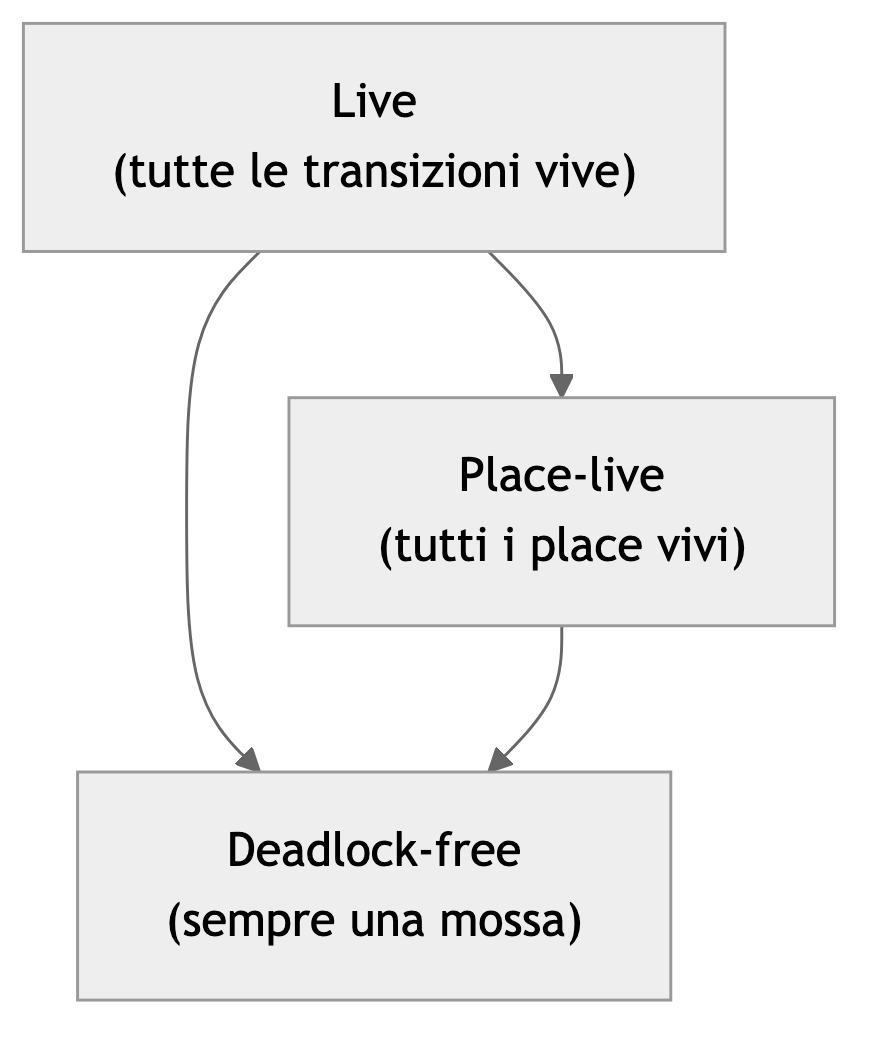
\includegraphics[width=0.54\linewidth,height=0.32\textheight,keepaspectratio]{images/mermaid/10_2.png}
\end{center}

\emph{Le frecce sono implicazioni; nessuna si inverte.}

\begin{boxnote}{Le implicazioni (e le NON-implicazioni)}
Valgono (per contrapposizione si leggono anche al negativo): - \textbf{live $\Longrightarrow$ place-live} — quindi \emph{non place-live $\Longrightarrow$ non live}. - \textbf{live $\Longrightarrow$ deadlock-free} — quindi \emph{possibile deadlock $\Longrightarrow$ non live}. - \textbf{place-live $\Longrightarrow$ deadlock-free} — quindi \emph{possibile deadlock $\Longrightarrow$ non place-live}. - $t$ \textbf{dead $\Longrightarrow$ non-live}; $p$ \textbf{dead $\Longrightarrow$ non place-live} (e $\Longrightarrow$ non live).

\textbf{Non} valgono (controesempi esistono): - deadlock-free $\centernot\{\Longrightarrow\}$ live (una rete può girare per sempre con una transizione morta). - deadlock-free $\centernot\{\Longrightarrow\}$ place-live. - place-live $\centernot\{\Longrightarrow\}$ live. - non-live $\centernot\{\Longrightarrow\}$ non place-live (una rete può avere una transizione dead ma tutti i place vivi).
\end{boxnote}

Queste proprietà — boundedness, liveness, deadlock-freedom — sono i primi mattoni dell'analisi comportamentale. Per verificarle su reti grandi, però, l'esplorazione dell'occurrence graph è costosa: nella prossima lezione introdurremo un approccio \textbf{algebrico}, basato sulle matrici, che permette di ragionare sulle reti senza costruire tutto lo spazio degli stati. $\rightarrow$ \hyperref[ch:11]{11 — Net Matrices}